\section{Architectures}

\begin{frame}
	\frametitle{Shallow architectures}
	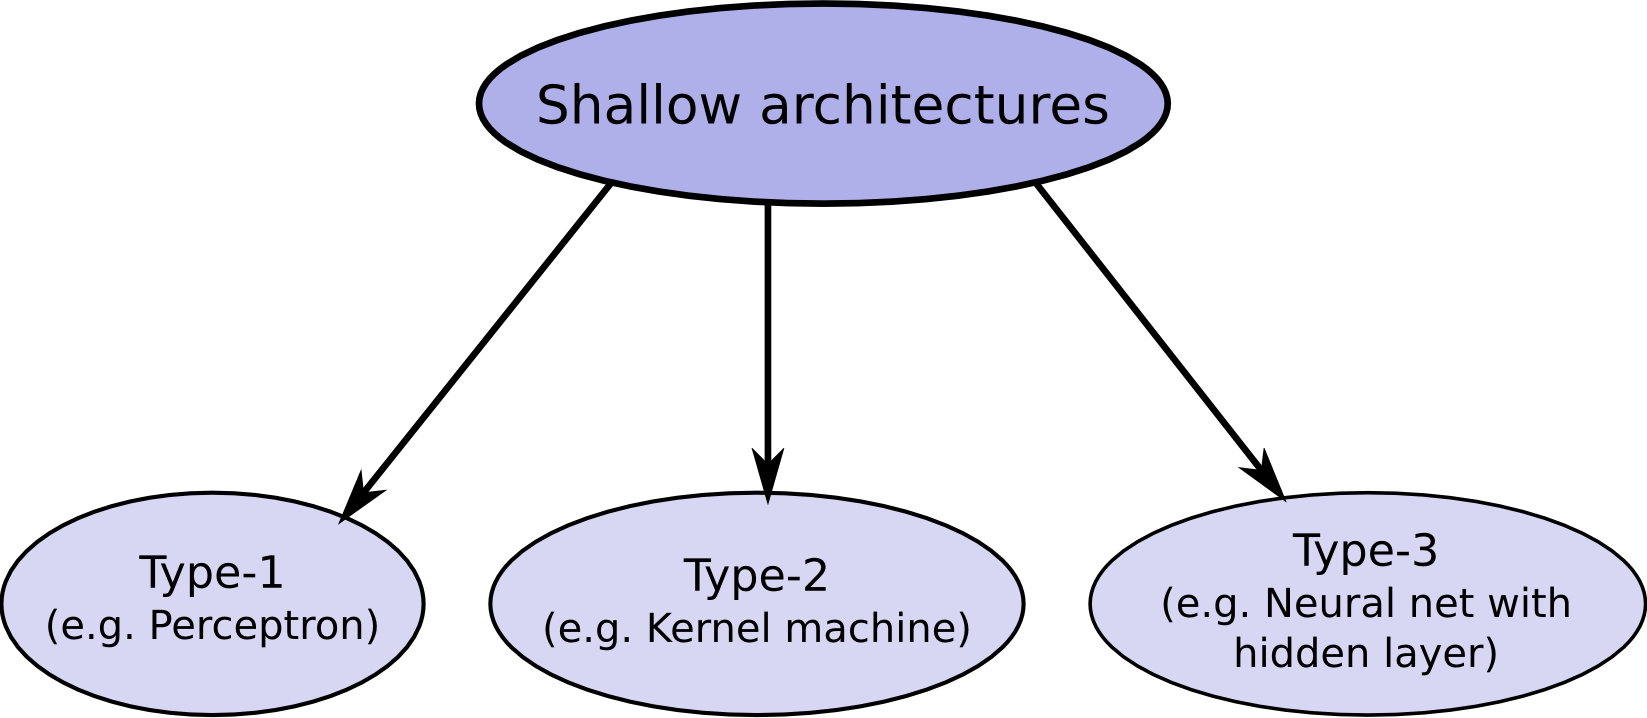
\includegraphics[width=10cm]{images/architectures.png}
\end{frame}

\begin{frame}
	\frametitle{Type-1 architectures}
	\begin{columns}
		\begin{column}{6.5cm}
			\begin{itemize}
				\item Fixed preprocessing and linear predictor
				\begin{displaymath}
					f(x)= \begin{cases}
						1& \text{if } b + \sum_{i=1}^{n}w_i \phi_i(x) > 0\\
						0& \text{else}
					\end{cases}
				\end{displaymath}
				$\phi_{i}$ $i$-th feature of preprocessing
				\item Preprocessing hand-crafted, thus task-specific
				\item Used in practical applications
			\end{itemize}
		\end{column}
		\begin{column}{5cm}
			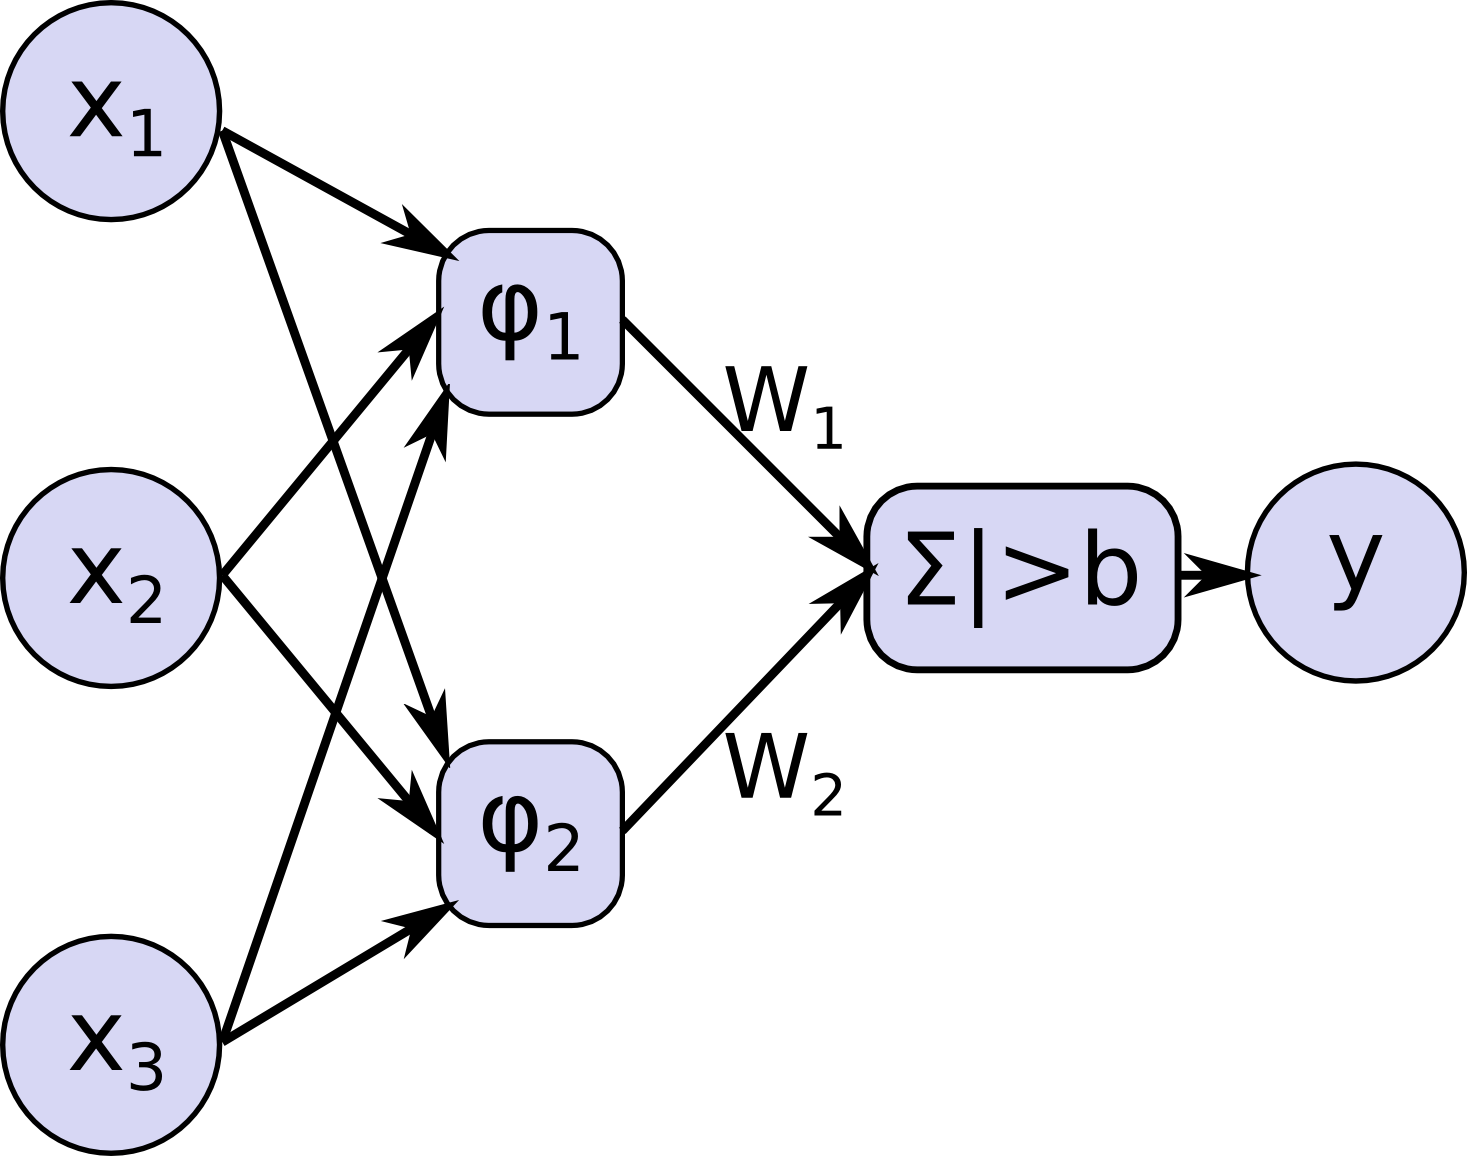
\includegraphics[width=5cm]{images/perceptron.png}
		\end{column}
	\end{columns}
\end{frame}

\begin{frame}
	\frametitle{Type-2 architectures}
	\begin{columns}
		\begin{column}{6.5cm}
			\begin{itemize}
				\item Template matchers and linear predictor
				\begin{displaymath}
					f(x)= \begin{cases}
						1& \text{if } b + \sum_{i=1}^{n}w_i K(x,x_i) > 0\\
						0& \text{else}
					\end{cases}
				\end{displaymath}
				$K(\cdot,\cdot)$ kernel function
				\item $K(\cdot,x_i)$ data dependent feature
				\item Often convex optimization program
				\note[item]{Margin loss, squared error}
			\end{itemize}
		\end{column}
		\begin{column}{5cm}
			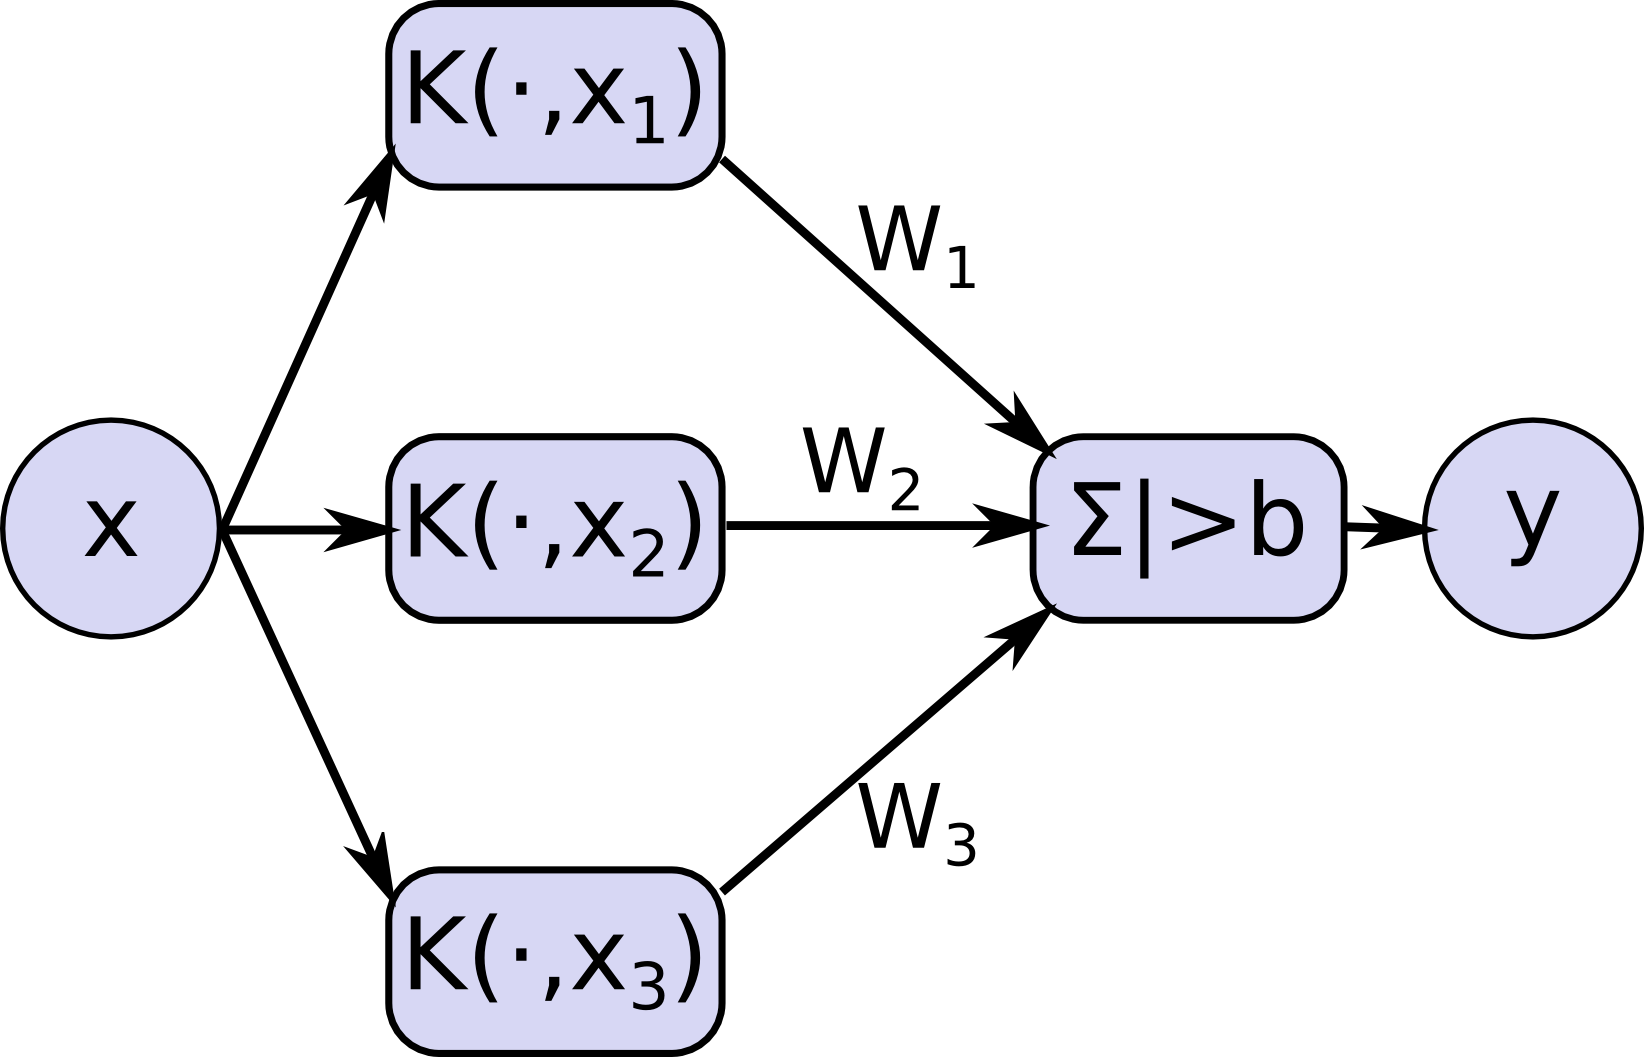
\includegraphics[width=5cm]{images/kernelMachine.png}
		\end{column}
	\end{columns}
\end{frame}

\begin{frame}
	\frametitle{Local kernels}
	\begin{columns}
		\begin{column}{7cm}
			\begin{definition}[Local kernel]
				A kernel is called \emph{local} iff $K(x,x_{i})>\rho$ only for some connected region around $x_i$.
			\end{definition}
			\begin{itemize}
				\item Example: Gaussian kernel $K(\mathbf{x},\mathbf{x}_i) =\exp{\left(-\frac{1}{2}\frac{\norm{\mathbf{x}-\mathbf{x}_i}^2_2}{\sigma^2}\right)}$
				\item Discrimination between points $\mathbf{x}$ close to $\mathbf{x}_i$ and not
				\item Local template matchers
				\item Algorithms: SVM, Gaussian processes, Nadaraya-Watson, Parzen windows, LLE, Isomap
			\end{itemize}
		\end{column}
		\begin{column}{4.5cm}
			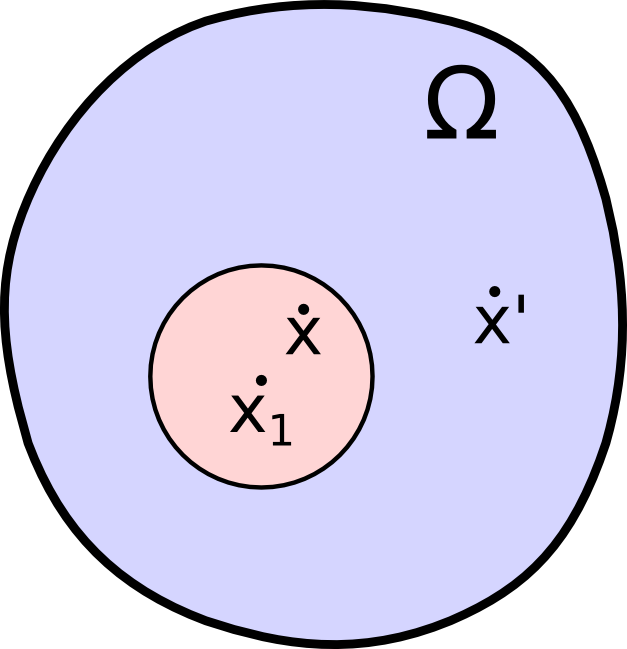
\includegraphics[width=4.5cm]{images/localKernel.png}
		\end{column}
	\end{columns}
\end{frame}

\begin{frame}
	\frametitle{Type-3 architectures}
\end{frame}

\begin{frame}
	\frametitle{Deep architectures}
\end{frame}
